% Ray tracing structures on the GPU has been mapped more or less 100%
% from CPU structures. We need to build them for the GPU instead. That
% means rethinking some of the algorithms (like add persistent
% threads.)



\chapter{Ray Tracing}\label{chp:rayTracing}

\chapterquote{Some argue that in the very long term, rendering may best be
  solved by some variant of ray tracing, in which huge numbers of rays sample
  the environment for the eye’s view of each frame. And there will also be
  colonies on Mars, underwater cities, and personal jet packs.}{Tomas Möller and
  Eric Haines}


% Motivate!

% An optimized ray tracer will be used to test whether or not more time
% spent on creating a better kD tree will pay off in final rendering
% time.

In this chapter we shall look at how to implement a ray tracer and how it can be
optimized to run efficiently on graphics hardware. The result will be an
optimized ray tracer, which will be used for evaluating the quality of kd-trees
in \refchapter{chp:results}.

A ray, $r$, is defined as a line which starts at its \textit{origin} and can be
traced infinitely along a certain \textit{direction}, so $r = \{origin,
direction\} \in \{R^3, R^3\}$. Before the actual ray tracing can be performed,
the primary rays traced from the camera and into the scene must first be
computed and stored in a Ray List, $rays$. How these rays can be generated is a
large topic in itself and lies outside the scope of this thesis. Chapter 4 in
\citebook{RTR3} provides good insight into the theory needed for creating the
primary rays.

The generel structure for a ray tracer that handles reflective surfaces can be
seen in \refalg{alg:generelRayTracer}. Each ray is independent of the other rays
and can therefore be traced in parallel by the GPU. The algorithm first
determines the closest intersecting triangle, i.e. the triangle first
\textit{seen} by the ray. It then computes the color of the point on the
triangle seen by the ray and blends it with the color in $pixels[r]$ that has
been accumulated so far. How the color is computed is not relevant to the
kd-tree quality results in \refchapter{chp:results} and is therefore discussed
in this thesis. Suffice it to say that the ray tracer produced as part of the
thesis uses the \textit{generel lighting equation} described on page 83 in
\citebook{RTR2}. Finally the algorithm checks if a triangle is reflective and if
it is then a reflection ray is generated and added to the $nextRays$ list. If
$nextRays$ contains one or more rays reflection rays, the process is repeated.

\begin{algorithm}
  \caption{A generel ray tracer.}
  \label{alg:generelRayTracer}
  \begin{algorithmic}
    \PROCEDURE{RayTracer}
              {$rays$ : Ray List, $scene$ : Scene, $pixels$ : Frame}
              {$pixels$ : Frame}{
                \PARALLELFOR{$r$}{$rays$}
                  \ASSIGN{$triangle$}{ClosestIntersection$(r, Scene)$}
                  \ASSIGN{$pixels[r]$}{ComputeColor$(pixels[r], r, triangle)$}
                  \DECLARE{$nextRays$}{Ray List}
                  \IF{IsReflective$(triangle)$}
                    \STATE{$nextRays$.Add(GenerateReflectionRay$(triangle, ray)$)}
                  \ENDIF
                \ENDFOR
                \IF{$nextRays$.NotEmpty}
                  \ASSIGN{$pixels$}{RayTracer$(nextRays, scene, pixels)$}
                \ENDIF
              }
  \end{algorithmic}
\end{algorithm}

In this chapter i will present two methods for determining which triangle in a
scene a ray intersects. In \refsection{sec:exhaustive} I present an exhaustive
ray tracer implementation, which find the closest intersection point by
comparing each ray with every triangle. In
\refsection{sec:hierarchicalTraversal} I then present a hierarchical ray tracer,
which will use the kd-tree to minimize the amount of triangles each ray needs to
be compared with. In the same section I will describe three optimizations that
can be applied to hierachical ray tracers running on GPU's. The optimizations
will be added incrementally to the hierarchical ray tracer and implementation
details to each specific optimization is therefore discussed alongside the
theory. The optimized ray tracer will use the short-stack optimization from
\horn, a packet scheme inspired by Wald et al.\citebook{Wald:2001:IRCRT} and an
optimization inspired by empty space maximizing, that utilizes a leaf's bounding
box data computed while creating the kd-tree.

The ray tracers and their optimization will be evaluated in
\refchapter{chp:results} and should show that the hierarchical ray tracer is
faster than the exhaustive ray tracer. This will be a very important result, as
the time spent rebuilding acceleration structures for dynamic scenes would
otherwise be wasted.

In \refsection{sec:exhaustive} and \refsection{sec:hierarchicalTraversal} I will
merely have assumed that a method exists for determining ray/triangle
intersection. In the final section of this chapter I will discuss two such
methods with respect to the GPU's memory hierarchy and maximizing
occupancy.



\section{Exhaustive Ray Tracing} \label{sec:exhaustive}

Before directing our focus on hierarchical ray tracers, we will first
take a look at an exhaustive ray tracer.

% GPU does bruteforcing well.

The reason that an exhaustive ray tracer is interesting is that the GPU comes
with high computational power, but little tolerance for branching, as was
discussed in \refsection{sec:threadHierarchy}. An exhaustive ray tracer fits
very well into such an architecture, since intersecting each ray with every
triangle certainly requires a lot of computational power, and every ray in a
warp will loop over the same triangles, so the triangle-loop will not cause
thread divergence.

% Algorithm

The exhaustive ray intersection algorithm is presented in
\refalg{alg:exhaustive}. The actual ray tracers implemented in this thesis also
compute and return the ray's barycentric coordinates on the triangle, presented
in \refsection{sec:intersection}, which is used for interpolating the normals at
the triangle's vertices across its surface and needed to perform lighting
calculations. But in order to keep the algorithms simple and instructive, this
has been omitted and is assumed to be performed by ComputeColor method in
\refalg{alg:generelRayTracer}.


\begin{algorithm}
  \caption{Exhaustive ray tracer}
  \label{alg:exhaustive}
  \begin{algorithmic}
    \PROCEDURE{Exhaustive}
              {$R$ : Ray, $Ts$, Triangle List}
              {$t_{near}$ : Triangle}{
                \ASSIGN{$t_{near}$}{$Ts[0]y$}
                \FOREACH{$t$}{$Ts$}
                  \ASSIGN{$t_{near}$}{ClosestIntersecting$(t, t_{near})$}
                \ENDFOR
              }
  \end{algorithmic}
\end{algorithm}

The downside to the exhaustive approach is that for $n$ rays and $m$
triangles the time complexity becomes $O(nm)$.

\section{Hierarchical Ray Tracing}\label{sec:hierarchicalTraversal}

% Time complexity of O(n log m)

Hierarchical ray tracers provide a better upper bound than exhaustive ray
tracers. Given a hierachical data structure over $m$ geometric primitives in a
scene, the nearest leaf node can be found in $O(\log m)$ time. For $n$ rays
this yields a time complexity of $O(n \log m)$, significantly better than the
exhaustive ray tracer from \refsection{sec:exhaustive}.

% Describe how the tree is traversed

When ray tracing a scene that has been divided by a kd-tree, each ray needs to
traverse the tree and find the nearest leaf node. At each interior node, the ray
needs to determine which of the children are closest and in front of the
ray. This child is then traversed next and the process is continued until a leaf
node is reached. The ray then needs to intersect each triangle in the leaf and
determine which intersected triangle, if any, is closest. If the ray intersects
a triangle, then it reports this intersection, if not then it needs to continue
traversing the tree. How this is done is the topic of \refsection{sec:kdRestart}
and \refsection{sec:shortStack}. The generel algorithm for ray tracing a kd-tree
can be seen in \refalg{alg:generelTracing}.

\begin{algorithm}
  \caption{A generel kd-tree traversal algorithm for ray tracing}
  \label{alg:generelTracing}
  \begin{algorithmic}
    \PROCEDURE{KDTraversal}
              {$ray$ : Ray, $tree$ : kd-tree}
              {$t_{near}$ : Triangle}{
                \WHILE{ray hasn't intersected}
                  \COMMENTIT{Traverse the tree until the closest leaf is found
                    and store the distance to the closest splitting
                    plane in $d_{split}$.}
                  \ASSIGN{$(leaf, d_{split})$}{TraverseTree($ray, tree$)}
                  \COMMENTIT{Intersect triangles in leaf and return
                    closest intersection.}
                  \ASSIGN{$d_{hit}$}{Intersect($ray, leaf.triangles$)}
                  \COMMENTIT{Break if a closest intersection
                    is found and return it.}
                  \IF{$d_{hit} < d_{split}$}
                    \ASSIGN{$t_{near}$}{Closest triangle in $leaf.triangles$}
                    \STATE{\textbf{break}}
                  \ELSE
                    \ASSIGN{$ray.origin$}{$ray.origin + d_{split} * ray.direction$}
                  \ENDIF
                \ENDWHILE
              }
  \end{algorithmic}
\end{algorithm}

% Traversal method

The method used to determine which of an interior node's children to visit next
can be seen in \refalg{alg:generelTraversal}. For each interior node the ray
first needs to determine which of the two children are placed \textit{nearest}
and \textit{farthest} along the rays direction. It then computes the signed
distance from the ray to the nodes splitting plane. If this distance is below 0
then the plane is located behind the ray and the farthest child must be
visited. If the distance is above 0 then the nearest node needs to be visited
next. In addition the distance, $d_{split}$ to the nearest splitting plane in
front of the ray needs to be updated. $d_{split}$ is used to advance the ray
beyond a visited leaf node if it did not intersect any primitives.

\begin{algorithm}
  \caption{A basic kd-tree traversal algorithm}
  \label{alg:generelTraversal}
  \begin{algorithmic}
    \PROCEDURE{Traversal}
              {$ray$ : Ray, $tree$ : kd-tree}
              {$leaf$ : Node, $d_{far}$ : Number}{
                \ASSIGN{$d_{far}$}{$\infty$}
                \ASSIGN{$node$}{$tree.root$}
                \WHILE{$node \neq LEAF$}
                  \COMMENTIT{The signed distance to the nodes splitting plane.}
                  \ASSIGN{$node_{near}$}{$ray.direction[node.axis] > 0$ ? $node.left$ : $node.right$}
                  \ASSIGN{$node_{far}$}{$ray.direction[node.axis] > 0$ ? $node.right$ : $node.left$}
                  \ASSIGN{$d_{split}$}{($node.splitValue - ray.origin[node.axis]) / ray.direction[node.axis]$}
                  \IF{$0 < d_{split}$}
                    \ASSIGN{$node$}{$node_{near}$}
                    \ASSIGN{$d_{far}$}{min$(d_{split}, d_{far})$}
                  \ELSE
                    \ASSIGN{$node$}{$node_{far}$}
                  \ENDIF
                \ENDWHILE
              }
  \end{algorithmic}
\end{algorithm}

In \reffig{fig:simpleScene} a simple scene consisting of 4 triangles
is shown. The corrosponding kd-tree matching the axis aligned
splitting planes is shown in \reffig{fig:simpleTree}. A tree traversal
of the ray, $R(t) = t \vectwoT{2}{1} + \vectwoT{0}{1}$, entering the
scene in the lower left would look like this: Upon entering the scene
the ray first visits the root node, 0. Node 0 splits the scene along
the x-axis at position 4 and the rays distance to that plane is then
$(4 - 0) / 2 = 2$. The ray therefore proceeds to the childnode $2 > 0$ 
? $1$ : $2 = 1$. The signed distance to node 1's splitting plane is $(4 -
1) / 1 = 3$ and the ray proceeds to node $1 > 0$ ? $3$ : $2 = 3$, where it
finds no primitives to intersect. The ray is then advance by the
minimum splitting distance, which was 2, and becomes $R'(t) = R(t) + 2
\vectwoT{2}{1} = t \vectwoT{2}{1} + \vectwoT{4}{3}$. Since the ray did
not intersect any geometry and has not advanced beyond the scene, the
traversal process is restarted for $R'(t)$.


\begin{figure}
  \centering
  \subfloat[A simple scene divided by a kd-tree.]{
    \begin{tikzpicture}[y=0.5cm, x=0.5cm,font=\sffamily]
      \drawNode{0,0}{8,0}{8,6}{0,6}

      % Tris
      \drawTri{0,6}{1,4}{2,5}
      \draw (1,5) node{0};
      \drawTri{4,6}{3,4}{2,5}
      \draw (3,5) node{1};
      \drawTri{4,2}{5,6}{6,4}
      \draw (5,4) node{2};
      \drawTri{8,0}{7,2}{6,1}
      \draw (7,1) node{3};

      % Splits
      \draw (4,0) -- (4,6);
      \draw (0,4) -- (4,4);
      \draw (2,4) -- (2,6);
      \draw (4,2) -- (8,2);

      % Ray
      \drawRay{0,1}{2,2}

      %axes
      \draw[->] (0,0) -- coordinate (x axis mid) (9,0);
      \draw[->] (0,0) -- coordinate (y axis mid) (0,7);
      %ticks
      \foreach \x in {0,2,...,9}
     		\draw (\x,1pt) -- (\x,-3pt)
			node[anchor=north] {\x};
    	\foreach \y in {0,2,...,7}
     		\draw (1pt,\y) -- (-3pt,\y) 
     			node[anchor=east] {\y}; 
    \end{tikzpicture}
    \label{fig:simpleScene}
  }
  \hspace{20pt}
  \subfloat[The kd-tree matching the scene. Nodes contain information
    about which axis have been divided and where. Leaf nodes contain a
    set of the triangles they overlap.]{
    \begin{tikzpicture}[y=0.5cm, x=.5cm,font=\sffamily,
        level/.style={sibling distance=40mm/#1}]
      \node [visitedNode] (0){$\begin{array}{c}0\\x:4\end{array}$}
        child {node [visitedNode] (1) {$\begin{array}{c}1\\y:4\end{array}$}
          child {node [visitedLeaf] (e) {$\begin{array}{c}3\\\emptyset\end{array}$}}
          child {node [node] (3) {$\begin{array}{c}4\\x:2\end{array}$}            
            child {node [leaf] (e) {$\begin{array}{c}7\\\{0\}\end{array}$}}
            child {node [leaf] (e) {$\begin{array}{c}8\\\{1\}\end{array}$}}
          }
        }
        child {node [node] (2) {$\begin{array}{c}2\\y:2\end{array}$}
            child {node [leaf] (e) {$\begin{array}{c}5\\\{2\}\end{array}$}}
            child {node [leaf] (e) {$\begin{array}{c}6\\\{3\}\end{array}$}}
        };
    \end{tikzpicture}
    \label{fig:simpleTree}
  }
  \caption[A simple scene and its kd-tree.]{}
  \label{fig:simpleSceneTree}
\end{figure}


\subsection{KD-restart}\label{sec:kdRestart}

% KD restart is the simplest and fastest.

The approach presented above, where kd-tree traversal is restarted at the root
node, is known as \textit{kd-restart} and is one of the simplest algorithms for
ray tracing kd-trees. The reason for the name is that if a ray does not
intersect any triangles in the nearest leaf node, then it advances past that
leaf node and restarts traversal from the root of the tree.

% Instead of advancing the ray simply update tMin

The algorithm in it's entirety is presented in \refalg{alg:KDRestart}. Instead
of advancing the ray by updating it's origin, a signed distance, $d_{min}$, is
used to determine how far a ray has traveled.

\begin{algorithm}
  \caption{KD Restart}
  \label{alg:KDRestart}
  \begin{algorithmic}
    \PROCEDURE{KDRestart}
              {$ray$ : Ray, $tree$ : kd-tree}
              {$t_{min}$ : Number}{
                \ASSIGN{$t_{min}$}{$0$}
                \WHILE{$t_{min} < \infty$}
                  \ASSIGN{$t_{next}$}{$\infty$}
                  \ASSIGN{$node$}{$tree.root$}
                  \COMMENTIT{Traverse the tree until a leaf node is reached}
                  \WHILE{$node \neq LEAF$}
                    \ASSIGN{$t_{split}$}{($node.splitValue - ray.origin[node.axis]) / ray.direction[node.axis]$}
                    \IF{$t_{min} < t_{split}$}
                      \ASSIGN{$node$}{$ray.direction[node.axis] > 0$ ? $node.left$ : $node.right$}
                      \ASSIGN{$t_{next}$}{min$(t_{split}, t_{next})$}
                    \ELSE
                      \ASSIGN{$node$}{$ray.direction[node.axis] > 0$ ? $node.right$ : $node.left$}
                    \ENDIF
                  \ENDWHILE
                  \COMMENTIT{Advance the ray to the next splitting plane.}
                  \ASSIGN{$t_{min}$}{$t_{next}$}
                  \COMMENTIT{Test intersection with the leafs primitives}
                  \FOREACH{$triangle$}{$node.triangles$}
                    \ASSIGN{$t_{min}$}{\MIN{$(t_{min}}{$\textbf{Intersect}$(triangle, ray))$}}
                  \ENDFOR
                  \IF{$t_{min} < t_{next}$}
                    \STATE{\textbf{break}}
                  \ENDIF
                \ENDWHILE
              }
  \end{algorithmic}
\end{algorithm}

\subsection{Short stack}\label{sec:shortStack}

% Kd-Restart traverses many of the same nodes, because 

When a ray triggers a restart in kd-restart, it will almost always traverse many
of the same tree nodes as it did in its previous traversel. The reason for this
is that kd-trees will often store spatially local nodes as local nodes in the
tree. CPU ray tracers solve this problem by pushing the not-visited child of an
interior node onto a stack and then restarting from the first node on that
stack. This can save a lot of resources otherwise spent on traversing the tree,
since the ray will now restart further down the kd-tree and closer to the next
leaf that should be visited.

CUDA's memory model, however, isn't flexible enough for this approach, which
requires either dynamically allocating more memory if the stack is filled or
pre-allocating a \textit{large enough} stack in local memory to handle any given
kd-tree, something that could require quite large amounts of memory for huge
scenes and might even require too much memory for practical use on todays
graphics cards. The solution proposed by \horn{} was to use a
\textit{short-stack}, a fixed-size, circular stack of $N$ elements, and then
revert to using kd-restart if the stack underflows. In their research they found
that a short-stack approach only visited 3\% more nodes compared to the
unlimited stack in CPU approaches.

% Only push usefull 'forward' nodes to the stack.

Obviously all child nodes can not be pushed onto the short-stack, as that would
force the rays to visit the entire kd-tree. Therefore restrictions need to be
formulated as to which nodes should be pushed onto the short-stack. The first
restriction is not to push nodes behind the ray, since the ray can never
intersect these. The second restriction is not to push nodes where the distance
to the splitting plane is greater than $d_{next}$, as these would never be
visited in a kd-restart traversal. The reasoning behind this is that if a ray
advances beyond the splitting plane of a higher interior node, it effectively
means the ray should never visit that nodes nearest subtree again and therefore
no nodes from that subtree should be stored in the short-stack. An
implementation of kd-restart with the short-stack optimization is shown in
\refalg{alg:ShortStack}.

\begin{algorithm}
  \caption{Short stack}
  \label{alg:ShortStack}
  \begin{algorithmic}
    \PROCEDURE{ShortStack}
              {$ray$ : Ray, $tree$ : kd-tree}
              {$t_{min}$ : Number}{
    \ASSIGN{$t_{min}$}{$0$}
    \WHILE{$t_{min} < \infty$}
      \IF{$stack$.IsEmpty}
        \ASSIGN{$node$}{$tree.root$}
        \ASSIGN{$t_{next}$}{$\infty$}
      \ELSE
        \ASSIGN{$(node, t_{next})$}{$stack$.Pop}
      \ENDIF
      \COMMENTIT{Traverse the tree until a leaf node is reached}
      \WHILE{$node \neq LEAF$}
        \ASSIGN{$t_{split}$}{($node.splitValue - ray.origin[node.axis]) / ray.direction[node.axis]$}
        \IF{$t_{min} < t_{split}$}
          \ASSIGN{$node$}{$ray.direction[node.axis] > 0$ ? $node.left$ : $node.right$}
          \IF{$t_{split} < t_{next}$}
            \STATE{stack.push($upperChild, t_{next}$)}
          \ENDIF
          \ASSIGN{$t_{next}$}{min$(t_{split}, t_{next})$}
        \ELSE
          \ASSIGN{$node$}{$ray.direction[node.axis] > 0$ ? $node.right$ : $node.left$}
        \ENDIF
      \ENDWHILE
      \COMMENTIT{Advance the ray to the next splitting plane.}
      \ASSIGN{$t_{min}$}{$t_{next}$}
      \COMMENTIT{Test intersection with the leafs primitives}
      \FOREACH{$triangle$}{$node.triangles$}
        \ASSIGN{$t_{min}$}{\MIN{$(t_{min}}{$\bf{Intersect}$(triangle, ray))$}}
      \ENDFOR
      \IF{$t_{min} < t_{next}$}
        \STATE{\textbf{break}}
      \ENDIF
    \ENDWHILE
              }
  \end{algorithmic}
\end{algorithm}

% Example

Let us look at a simple example of how the short-stack will speedup
traversal. Using the scene in \reffig{fig:simpleSceneTree} again, we saw
previously that the ray, $R(t) = t \vectwoT{2}{1} + \vectwoT{0}{1}$, will
traverse nodes 0, 1, and 3. At node 0 the distance to the splitting plane was 2,
meaning the splitting plane is in front and the child not traversed should be
pushed to the short-stack. At node 1 the distance was 3, so the ray intersects
node 1's splitting plane after node 0's. Node 1's other child therefore doesn't
need to be pushed to the stack. The result of the first traversal can be seen on
\reffig{fig:shortStack1}.

So far the short-stack traversal and kd-restart traversal have both choosen the
exact same path through the tree. But where kd-restart would have had to restart
its traversal from the root node, the short-stack allows the ray to start the
second traversal from node 2 and proceed to leaf 5, where the ray intersects
triangle 2.

In this simple example having a short-stack only allows the ray to skip one node
at the cost of maintaining and using a short-stack, which will cause a
significant overhead. Consequently having a short-stack will probably not provide any
speedup in this small example. But imagine this simple tree as a subtree in a
much larger scene, with perhaps 10 levels of nodes above it. Then a short-stack
implementation allows the ray to skip those first 11 nodes, which can yield
quite a performance improvement.

\begin{figure}
  \centering

  \subfloat[The short stack algorithm's first traversal of the scene
    from \reffig{fig:simpleSceneTree}. When the ray traversed node 0
    it pushed  node 2 onto the short-stack.]{
    \begin{tikzpicture}[y=0.5cm, x=.5cm,font=\sffamily,
        level/.style={sibling distance=40mm/#1}]
      \node [visitedNode] (0){$\begin{array}{c}0\\x:4\end{array}$}
        child {node [visitedNode] (1) {$\begin{array}{c}1\\y:4\end{array}$}
          child {node [visitedLeaf] (e) {$\begin{array}{c}3\\\emptyset\end{array}$}}
          child {node [node] (3) {$\begin{array}{c}4\\x:2\end{array}$}            
            child {node [leaf] (e) {$\begin{array}{c}7\\\{0\}\end{array}$}}
            child {node [leaf] (e) {$\begin{array}{c}8\\\{1\}\end{array}$}}
          }
        }
        child {node [node] (2) {$\begin{array}{c}2\\y:2\end{array}$}
            child {node [leaf] (e) {$\begin{array}{c}5\\\{2\}\end{array}$}}
            child {node [leaf] (e) {$\begin{array}{c}6\\\{3\}\end{array}$}}
        };
                        
      % Short stack
      \draw (10,-4.5) -- (10,-7.5) -- (12,-7.5) -- (12,-4.5) -- (10,-4.5);
      \draw (10, -6.5) -- (12, -6.5);
      \draw (10, -5.5) -- (12, -5.5);
      \draw (11, -7) node{2};
      \draw (11, -6) node{-};
      \draw (11, -5) node{-};
    \end{tikzpicture}
    \label{fig:shortStack1}
  }
  \\
  \subfloat[The short stack algorithm's second traversal of the scene
    from \reffig{fig:simpleSceneTree}. Traversal starts from the first
    node on the stack, which is 2.]{
    \begin{tikzpicture}[y=0.5cm, x=.5cm,font=\sffamily,
        level/.style={sibling distance=40mm/#1}]
      \node [node] (0){$\begin{array}{c}0\\x:4\end{array}$}
        child {node [node] (1) {$\begin{array}{c}1\\y:4\end{array}$}
          child {node [leaf] (e) {$\begin{array}{c}3\\\emptyset\end{array}$}}
          child {node [node] (3) {$\begin{array}{c}4\\x:2\end{array}$}            
            child {node [leaf] (e) {$\begin{array}{c}7\\\{0\}\end{array}$}}
            child {node [leaf] (e) {$\begin{array}{c}8\\\{1\}\end{array}$}}
          }
        }
        child {node [visitedNode] (2) {$\begin{array}{c}2\\y:2\end{array}$}
            child {node [visitedLeaf] (e) {$\begin{array}{c}5\\\{2\}\end{array}$}}
            child {node [leaf] (e) {$\begin{array}{c}6\\\{3\}\end{array}$}}
        };
                        
      % Short stack
      \draw (10,-4.5) -- (10,-7.5) -- (12,-7.5) -- (12,-4.5) -- (10,-4.5);
      \draw (10, -6.5) -- (12, -6.5);
      \draw (10, -5.5) -- (12, -5.5);
      \draw (11, -7) node{-};
      \draw (11, -6) node{-};
      \draw (11, -5) node{-};
    \end{tikzpicture}
    \label{fig:shortStack2}
  }
  \caption[Short-stack kd-tree traversal.]{}
\end{figure}


\subsection{Packets}

% Packets: 2x2 packets on the CPU for to take advantage of SIMD
% instructions (Wald), warp size packets on the GPU. While
% \citebook{1230129} implemented packets, they merely assumed it would
% yield a speedup and did not provide any results. Aila2009 is against
% packets as they in practice seem to make it slower.

Using some form of \textit{packets} to accelerate ray tracing is quite
a standard technique. Packets where introduced to CPU ray tracers by
Wald et al.\citebook{Wald:2001:IRCRT}, who utilized
\textit{SIMD}\footnote{Single instruction, multiple data.}
instructions to trace four rays at a time. \horn{} extended the
short-stack approach with packet tracing, where individual threads
would trace multiple rays at a time to amortize the cost of traversing
the tree. Unfortunatly tracing several rays in one thread increases
thread incoherence across warps and \aila{} concludes that

\quotebook{It is worth noticing that [kd-restart] is faster than
  packet traversal in all cases, and with diffuse rays the difference
  is approximately 2X.}{Aila2009}

% As ray tracing becomes more complex packets also become less
% effective, as rays will become more chaotic in nature and less
% likely to fit into packets.

% I will adobt a pretty cheap packet strategy: I will trace my rays in
% 4x8 packets to increase (spatial) ray coherence across warps.

While \horn's approach to packet tracing might not have yielded the intended
increase in performance, the warp constructions likeness to SIMD means that the
GPU is already performing packet tracing. Instead of 4 rays per instruction, as
is the case with SIMD, a warp will trace rays in packets of 32 at a time on
current hardware.

The rays are stored in rows from left to right in a linear array. Performing a
\textit{sequantial ray/warp tracing} results in the ray/warp classification seen
in \reffig{fig:sequentialRayWarp} for an image with a resolution of 64x48. As
seen on the figure, a large number of warps are intersecting the detailed dragon
geometry. The threads in those warps who quickly intersect their rays with the
simple box will then have to idle, while waiting for the rays intersecting the
detailed dragon to finish.

Instead I propose to take advantage of the spatial coherence between
neighbouring rays and structure them in warpsized screenspace packets as done in
\reffig{fig:coherentRayWarp}. As the figure demonstrates not only does fewer
warps ray trace the detailed dragon, but the spatial coherence between the rays
in a warp causes more warps to ray trace only spatially local geometry.

\begin{figure}
  \subfloat[Sequential ray/warp tracing. Notice how almost all of the
    warps overlap both the dragon and box.]{
    \begin{tikzpicture}[y=0.45cm, x=.45cm,font=\sffamily]
      \node {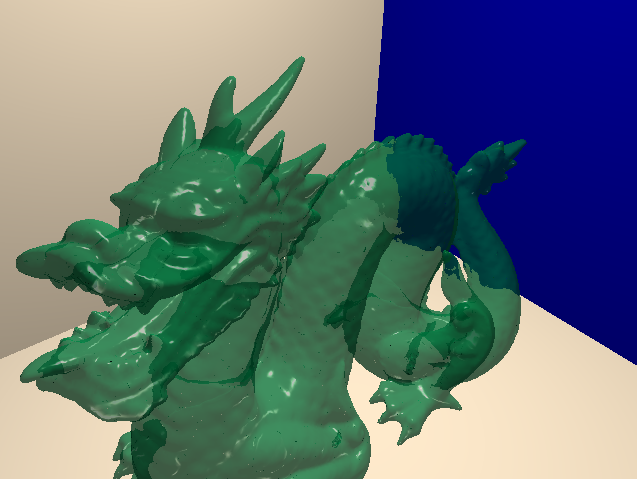
\includegraphics[width=7.2cm, height=5.4cm]{RefractionDragon}};
      \foreach \x in {-8,0,...,8} \draw (\x,-6) -- (\x, 6);
      \foreach \y in {-6,-5.75,...,6} \draw (-8,\y) -- (8, \y);
    \end{tikzpicture}
    \label{fig:sequentialRayWarp}
  }
  \hspace{20pt}
  \subfloat[Spatially coherent ray/warp tracing. Fewer warps will now
    ray trace the dragon and the spatial coherence between rays
    results in entire warps raytracing the same side of the box.]{
    \begin{tikzpicture}[y=0.45cm, x=.45cm,font=\sffamily]
      \node {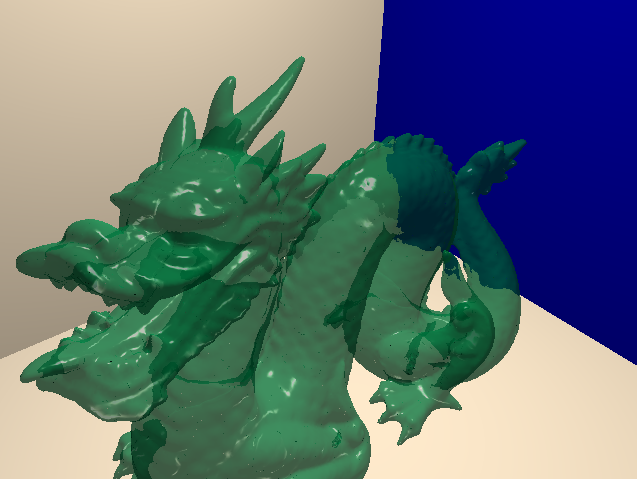
\includegraphics[width=7.2cm, height=5.4cm]{RefractionDragon}};
      \foreach \x in {-8,-7,...,8} \draw (\x,-6) -- (\x, 6);
      \foreach \y in {-6,-4,...,6} \draw (-8,\y) -- (8, \y);
    \end{tikzpicture}
    \label{fig:coherentRayWarp}
  }
  \caption[Sequantial and spatially coherent rays per warp.]{}
\end{figure}

The calculations needed to transform sequential ray ids into packeted ray ids
are quite simple and can be seen in \refalg{alg:packet}, but the performance
benefits of tracing coherent rays and sharing fetched global data among the rays
in a warp are enormous, as seen in \reffig{fig:rayTracerEvaluation}.

It should be noted that there exists a possibility that rays reflected multiple
times may eventually diverge completely and no longer be spatially coherent, but
this is no more of a problem than with the sequential ray/warp approach and the
screen packets will still speed up primary rays.

\begin{algorithm}
  \caption{Converting a thread id to a ray id.}
  \label{alg:packet}
  \begin{algorithmic}
    \PROCEDURE{PacketID}
              {$thread$ : id}
              {$ray$ : id}
              {\ASSIGN{$p$}{$thread / (p_{width} * p_{height})$}
                \ASSIGN{$grid_x$}{$p \mod  (image_{width} / p_{width})$}
                \ASSIGN{$grid_y$}{$p / (image_{width} / p_{width})$}
                \ASSIGN{$p_x$}{$threads \mod  p_{width}$}
                \ASSIGN{$p_y$}{$(threads \mod (p_{width} * p_{height})) / p_{width}$}
                \ASSIGN{$ray_x$}{$grid_x * p_{width} + p_x$}
                \ASSIGN{$ray_y$}{$grid_y * p_{height} + p_y$}
                \ASSIGN{$ray$}{$ray_x + ray_y * screen_{width}$}
              }
  \end{algorithmic}
\end{algorithm}


\subsection{Skipping Leaf Nodes}

% Inspired by empty space maximizing

The final ray tracer optimization presented in this thesis is inspired by the
early out option provided by empty space maximization.

%% and combines the simple traversal of kd-trees with the bvh-tree's rigorous
%% intersection checks.

Since the only information available to ray traversing a kd-tree is the position
of the splitting plane and not the bounding volume of the node, the ray can
easily get sidetracked and end up in leaf nodes, whose bounding box it does not
even intersect. \Reffig{fig:waywardRay} is a simple example of this. Extending
the ray, $R(t) = t \vectwoT{1}{1} + \vectwoT{-4}{0}$, we can clearly see that it
will intersect leaf node 2. Unfortunatly, when using kd-trees, the only
information available to the ray is that the node is split along the y-axis at
position 3, which means it needs to check everything below $y=3$ for
intersection. This is a problem in scenes with large empty areas that a ray has
to traverse. Each time the ray intersects a splitting plane in those empty
areas, it can get sidetracked and traverse subtrees that it does not
intersect. An example of this is the great hall in the Sponza scene, where
applying this optimization will yield quite a performance increase, as evidenced
in \reffig{fig:rayTracerEvaluation}.

Empty space maximization has shown us that providing an early out option for
rays that would otherwise get sidetracked can increase performance substantially
and that also applies to this case. Since the leafs bounding box is known from
the tree creation phase, it can be used to quickly skip leafs that the ray does
not intersect and save a ray lots of triangle intersection testing.

This optimization is not possible with the kd-tree alone and will thus not be a
solution to static geometry, where the kd-tree is only calculated once and
superfluous information is disgarded, such as the bounding box and parent
node. Another solution to diverging rays is presented under Future Work in
\refchapter{chp:future}.

\begin{figure}
  \centering
  \subfloat{
    \begin{tikzpicture}[y=0.5cm, x=.5cm]
      \drawNode{0,0}{6,0}{6,6}{0,6}      

      %Splits
      \draw (0,3) -- (6,3);
      
      % Leaf names
      \draw (3,1.5) node[leaf]{1};
      \draw (3,4.5) node[leaf]{2};

      \axes{7}{7}

      \drawRay{-4,0}{-3,1}
      \draw[line width=0.75pt, dashed, ->, color=gray] (-3,1) -- (0,4);
    \end{tikzpicture}
    \label{fig:waywardScene}
  }
  \subfloat{
    \begin{tikzpicture}[y=0.5cm, x=.5cm,font=\sffamily,
        level/.style={sibling distance=25mm/#1}]
      \node [visitedNode] (0){$y:3$}
        child {node [visitedLeaf] (1) {1}}
        child {node [leaf] (2) {2}}
        ;
    \end{tikzpicture}
    \label{fig:waywardTree}
  }
  \caption{A ray straying into a tree node, whose bounding box it does
    not intersect.}
  \label{fig:waywardRay}
\end{figure}

% Is not a generel kd-tree optimization. Only works because we already
% have the bounding boxes from the tree creation phase and won't
% deallocate the space.




\section{Ray/Triangle Intersection}\label{sec:intersection}

The inherent diverging behaviour of rays traversing the kd-tree makes them hard
to parallize efficiently on the graphics card, since data access will be nearly
impossible to coallesce. The solution is to have enough active warps to
effectively hide the latency from global data fetching. This means that each
rays register usage must be kept to a minimum, in order to have room for as many
active warps as possible.

Deciding which ray/triangle intersection method to use when ray tracing can both
lower register usage and yield a significant performance boost.

% Consists of 2 parts. Ray/plane intersection which tells us the
% distance the ray will travel, and ray/triangle tests which tells us
% if the ray intersected the triangle.

Ray/triangle intersection can be broken down into 2 parts: A \textit{ray/plane
  intersection} test, which computes the signed distance, $t$ a ray must travel
to intersect the plane spanned by a triangle, and a \textit{triangle inclusion}
test, which checks if the intersection point is located inside the triangle. The
inclussion test is usually performed by calculating the intersection points
\textit{barycentric coordinates} within the triangle.

Every point on a triangle, $T$, with vertices $a$, $b$ and $c$, can be described
as

\begin{displaymath}
  T(u,v) = (1-u-v)a + ub + vc, 0 \le u, 0 \le v, u+v \le 1
\end{displaymath}
 
where $(u, v)$ are the aforementioned barycentric coordinates. For a barycentric
coordinate to be inside $T$ it must therefore fulfill the requirements $0 \le
u$, $0 \le v$ and $u+v \le 1$.

Just as barycentric coordinates are used to linearly interpolate the vertex
positions across the triangle, they are also important for interpolating other
vertex attributes, such as normals or colors.

The following 2 ray/triangle intersection methods both compute the signed
distance and barycentric coordinates.

\subsection{Möller-Trumbore}

% One of the most popular intersection algorithms and featured in
% Real-Time Rendering.

The algorithm presented in Möller-Trumbore\citebook{MollerTrumbore97} is one of
the most popular algorithms for ray/triangle intersection, probably in no small
part due to its appearence in chapter 16.8 of Real-Time
Rendering\citebook{RTR3}, but also because it is one of the fastest ray/triangle
intersection algorithms that do not rely on extra memory and/or precomputations.

% Calculates the transformation that transform the triangle into the
% unit triangle and applies this transformation to the ray.

\fixme{This sounds more like woop does it not?}

The basic idea of the algorithm is to find the affine transformation
that, when applied to the triangle $T(u,v)$, transforms it into the unit
triangle, $U$, which has vertices $\vecthreeT{0}{0}{0}$,
$\vecthreeT{1}{0}{0}$ and $\vecthreeT{0}{1}{0}$. That affine
transformation is then applied to the ray, $R(t) = O + tD$, which
yields the vector $\vecthreeT{t}{u}{v}$, where $t$ is the distance to
the plane spanned by $T(u,v)$ and $u$ and $v$ are the barycentric
coordinates of the intersection point.

In short this boils down to solving the linear system of equations,
the \textit{ray/triangle intersection equation}

\begin{displaymath}
  \begin{array}{rl}
    & R(t) = T(u,v) \\
    \Updownarrow \\
    & O + tD = (1-u-v)a + ub + vc \\
  \end{array}
\end{displaymath}


Solving the ray/triangle intersection equation amounts to determining the signed
distance from the ray to the triangle, $t$, and the barycentric coordinates,
$(u, v)$. In \citebook{MollerTrumbore97} this is done by rearranging the terms
and applying Cramer's Rule, and the solution then becomes

\begin{displaymath}
  \vecthree{t}{u}{v} = \frac{1}{P \cdot E_1} 
  \vecthree{Q \cdot E_2}{P \cdot T}{Q \cdot D}
\end{displaymath}

where $E_1 = b - a$, $E_2 = c - a$, $T = O - a$, $P = D \times  E_2$
and $Q = T \times  E_1$.

\subsubsection{Implementation}

The implementation of this method is pretty straightforward using CUDA's vector
primitives and can be seen in \refalg{alg:moellerTrumbore}. The implementation
provided in \citebook{MollerTrumbore97} was optimized for the CPU and therefore
provided a lot of early out options as soon as the algorithm detects that a ray
has missed the triangle. Due to the wide SIMT architecture of GPUs, providing as
many early out possibilities as \citebook{MollerTrumbore97} causes a branching
overhead and results in reduced performance. This is understandable since only
one ray needs to intersect its triangle in order for the entire warp to perform
the complete intersection testing. For the ray tracers implemented as part of
this thesis the sweet spot was found to be only providing one early exit after
the ray/plane intersection and before copmuting the barycentric coordinates.

\begin{algorithm}
  \caption{Möller-Trumbore ray/triangle intersection test}
  \label{alg:moellerTrumbore}
  \begin{algorithmic}
    \PROCEDURE{Möller-Trumbore}
              {$T$ : triangle, $R$ : ray}
              {$hit$ : bool, $t$ : distance, $(u,v)$ : barycentric coordinates}
              {\ASSIGN{$E_1$}{$T.b - T.a$}
                \ASSIGN{$E_2$}{$T.c - T.a$}
                \ASSIGN{$T$}{$R.O - T.a$}
                \ASSIGN{$P$}{$R.D - E_2$}
                \ASSIGN{$Q$}{$T - E_1$}
                \ASSIGN{$determinant$}{$P \cdot E_1$}
                \ASSIGN{$t$}{$(Q \cdot E_2) / determinant$}
                \COMMENTIT{Provide early out if the triangle is behind
                  the ray.}
                \IF{$0 < t$}
                  \ASSIGN{$u$}{$(P \cdot T) / determinant$}
                  \ASSIGN{$v$}{$(Q \cdot R.D) / determinant$}
                  \ASSIGN{$hit$}{$0 \le u$ \textbf{and} $0 \le v$
                    \textbf{and} $u+v \le 1$}
                \ELSE
                  \ASSIGN{$hit$}{$false$}
                \ENDIF
              }
  \end{algorithmic}
\end{algorithm}


\subsection{Woop}

% Why Woop is better

While Möller-Trumbore's ray/triangle intersection approach requires minimal
storage, in the sense that it takes as input the vertex positions already stored
in global memory, it does unfortunatly require quite a lot of registers, since
it needs to both store the ray's parameters aswell as the determinant and the
matrix $\vecthreeT{Q \cdot E_2}{P \cdot T}{Q \cdot D}$. The high register usage
can be remedied by performing precalulations per triangle as described in
Chapter 5 of Sven Woops diploma thesis\citebook{woop:04:diplom}. The trade-off
is a higher per triangle storage requirement of the scene's geometry.

% Also translates the ray using the unit triangle.

As was the case with the Möller-Trumbore approach, Woops approach also
transforms the generel ray/triangle intersection problem into a
ray/unit triangle intersection problem, where the solution is
trivially calculated.

He observed that the triangle, $T$, can be transformed into the unit
triangle, $U$, by applying an affine transformation, consisting of a rotation
matrix, $m$, and a translation, $n$, on each of $T$'s vertices, $v$.

\begin{displaymath}
  U_v = m T_v + n, v \in \{a, b, c\}
\end{displaymath}

The inverse affine transformation is the one that transforms the unit
triangle into $T$.

\begin{displaymath}
  T_v = m' U_v + n', v \in \{a, b, c\}, m' = m^{-1}, n' = -m^{-1}n
\end{displaymath}

Given that we already know $T$ and $U$, $m'$ and $n'$ can be
constructed as follows

\begin{displaymath}
  m' = \left[ T_a - T_c, T_b - T_c, (T_a - T_c) \times (T_b - T_c)
    \right],
  n = T_c
\end{displaymath}

We can then derive $m$ and $n$ from $m'$ and $n'$. 

\begin{displaymath}
  m = (m')^{-1},
  n = - m n'
\end{displaymath}

This requires $m'$ to be invertable, which it always is for
\textit{non-degenerate triangles}\footnote{A degenerate triangles is
  a triangles that has collapsed into a line or a point.}.

%% Applying the affine transformation described by $m$ and $n$ to the
%% ray/triangle intersection equation we get

%% \begin{displaymath}
%%   \begin{array}{rl}
%%     & m R(t) + n = m T(u,v) + n\\
%%     \Updownarrow \\
%%     & m (O + tD) + n = m ((1-u-v)a + ub + vc) + n \\
%%     \Updownarrow \\
%%     & m (O + tD) + n = (1-u-v)U_a + u U_b + v U_c \\
%%   \end{array}
%% \end{displaymath}

Applying the affine transformation described by $m$ and $n$ to the
ray, $m * R(t) + n = R'(t) = tD' + O'$, it is transformed into the
same space as the unit triangle. Computing the distance, $t$, and
barycentric coordinates, $(u,v)$ then becomes trivial.

\begin{displaymath}
  \begin{array}{l}
    t = - D'_z / O'_z \\
    u = t D'_x + O'_x \\
    v = t D'_y + O'_y
  \end{array}
\end{displaymath}

Since each dimension in $R'$ can be computed independently, we get 

\begin{displaymath}
  \begin{array}{l}
    t = - (m_z \cdot D + n_z) / (m_z \cdot O) \\
    u = t (m_x \cdot D + n_x) + m_x \cdot O \\
    u = t (m_y \cdot D + n_y) + m_y \cdot O \\
  \end{array}
\end{displaymath}

where $m_i$ is the i'th row of $m$.

\subsubsection{Implementation}

The implementation is strightforward. $m$ and $n$ are computed and stored in 4
component vectors as $w_i = \left[m_i, n_i \right]$ prior to ray tracing. During
ray/triangle intersection each $w_i$ vector can then be loaded into register
memory one vector at a time. Compared to the Möller-Trumbore approach this saves
3 registers and can yield a sizeable performance increase, as can be seen in
\reffig{fig:rayTracerEvaluation}.

% early out

As in the implementation of Möller-Trumbore, the Woop implementation also only
has one early out option, which is placed right after the distance calculation.

% The extra space used by the precalcultations can be mitigated if the vertices
% are no longer needed.

Finally, the extra memory required for precalculating $m$ and $n$ can be
mitigated if the triangles vertex positions are replaced by $m$. This is only
possible however, if the vertices are not used elsewhere in the ray tracer.

